\documentclass{beamer}
\usepackage[utf8]{inputenc}
\usepackage[T1]{fontenc}
\usepackage[russian]{babel}
\usepackage{graphicx}
\usepackage{tikz}
\usecolortheme{orchid}
\title[World development indicators]{\Huge{World development indicators}}
\author[Moawad, Commandi, Isaeva, Schiavon, Snesarevskii] {{\Large Group 12:\\}Stefano Moawad\\Leonardo Commandi\\Diana Isaeva\\Andrea Schiavon\\Viktor Snesarevskii}
\date{April-May 2017}
\usebackgroundtemplate{\tikz\node[opacity=0.3] {\vbox to \paperheight{\vfil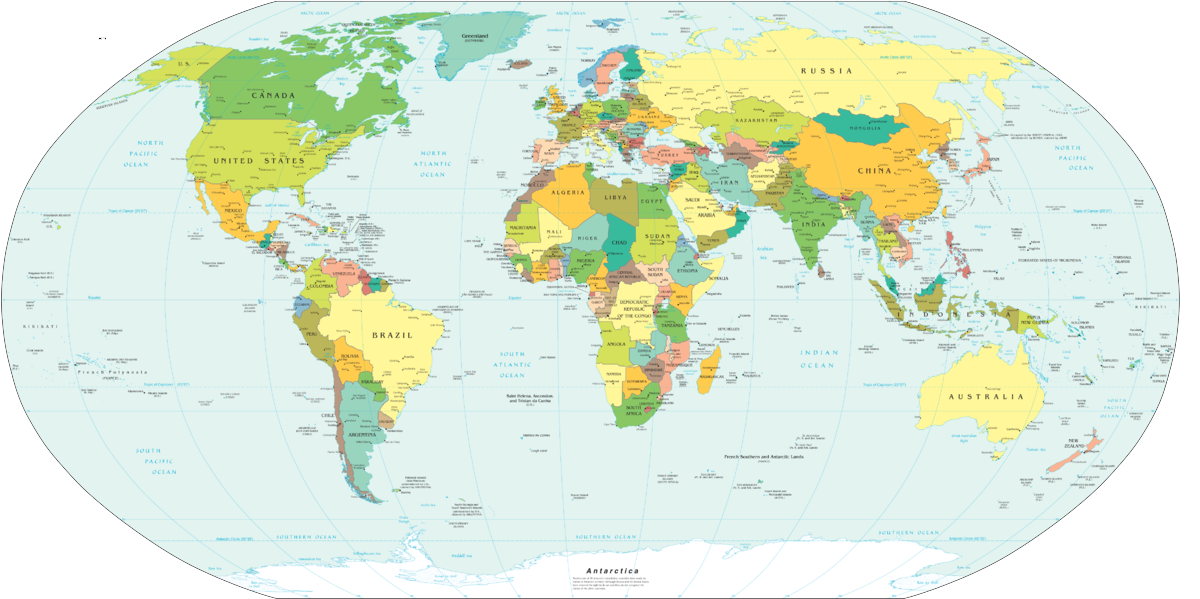
\includegraphics[width=\paperwidth]{map}\vfil}};}

\begin{document}
\frame{\titlepage}

\begin{frame}{Raw dataset}
\begin{block}{Indicators}
\scriptsize
\begin{tabular}{*{6}{l}}
Country name &
\only<1-1>{Country code}\only<2->{\!\!\tikz[baseline]\node[anchor=base,draw=red]{Country code};}& 
Indicator name & Indicator code & Year & 
\only<1-1>{Value}\only<2->{\!\!\tikz[baseline]\node[anchor=base,draw=cyan]{Value};}
\end{tabular}
\end{block}
\begin{block}{Country}
\scriptsize
\begin{tabular}{*{5}{l}}
\only<1-1>{Country code}\only<2->{\!\!\tikz[baseline]\node[anchor=base,draw=red]{Country code};}& 
Short name & Table name & Long name & Alpha 2 code \\[.15cm]
Currency unit & Special notes &
\only<1-1>{Region}\only<2->{\!\!\tikz[baseline]\node[anchor=base,draw=green]{Region};}&
Indice group & \textbf{etc...}
\end{tabular}
\end{block}

\begin{block}{Country notes}
\scriptsize
\begin{tabular}{*{5}{l}}
\only<1-1>{Country code}\only<2->{\!\!\tikz[baseline]\node[anchor=base,draw=red]{Country code};}&
\only<1-1>{Series code}\only<2->{\!\!\tikz[baseline]\node[anchor=base,draw=blue]{Series code};}&
Description
\end{tabular}
\end{block}
\begin{block}{Series}
\scriptsize
\begin{tabular}{*{5}{l}}
\only<1-1>{Series code}\only<2->{\!\!\tikz[baseline]\node[anchor=base,draw=blue]{Series code};}&
Topic & Indicator name\!\! & Short definition\!\! & Long definition \\[.15cm]
\only<1-1>{Unit of measure}\only<2->{\!\!\tikz[baseline]\node[anchor=base,draw=orange]{Unit of measure};}&
Periodicity & Base period & Other notes & \textbf{etc...}
\end{tabular}
\end{block}
\begin{block}{Series notes}
\scriptsize
\begin{tabular}{*{5}{l}}
\only<1-1>{Series code}\only<2->{\!\!\tikz[baseline]\node[anchor=base,draw=blue]{Series code};}&
\only<1-1>{Year}\only<2->{\!\!\tikz[baseline]\node[anchor=base,draw=black]{Year};}&
Description
\end{tabular}
\end{block}
\end{frame}


\end{document}